\documentclass[
  bibliography=totoc,     % Literatur im Inhaltsverzeichnis
  captions=tableheading,  % Tabellenüberschriften
  titlepage=firstiscover, % Titelseite ist Deckblatt
]{scrartcl}

% Paket float verbessern
\usepackage{scrhack}

% Warnung, falls nochmal kompiliert werden muss
\usepackage[aux]{rerunfilecheck}

% unverzichtbare Mathe-Befehle
\usepackage{amsmath}
% viele Mathe-Symbole
\usepackage{amssymb}
% Erweiterungen für amsmath
\usepackage{mathtools}

% Fonteinstellungen
\usepackage{fontspec}
% Latin Modern Fonts werden automatisch geladen
% Alternativ zum Beispiel:
%\setromanfont{Libertinus Serif}
%\setsansfont{Libertinus Sans}
%\setmonofont{Libertinus Mono}

% Wenn man andere Schriftarten gesetzt hat,
% sollte man das Seiten-Layout neu berechnen lassen
\recalctypearea{}

% deutsche Spracheinstellungen
\usepackage[ngerman]{babel}


\usepackage[
  math-style=ISO,    % ┐
  bold-style=ISO,    % │
  sans-style=italic, % │ ISO-Standard folgen
  nabla=upright,     % │
  partial=upright,   % │
  mathrm=sym,        % ┘
  warnings-off={           % ┐
    mathtools-colon,       % │ unnötige Warnungen ausschalten
    mathtools-overbracket, % │
  },                       % ┘
]{unicode-math}

% traditionelle Fonts für Mathematik
\setmathfont{Latin Modern Math}
% Alternativ zum Beispiel:
%\setmathfont{Libertinus Math}

\setmathfont{XITS Math}[range={scr, bfscr}]
\setmathfont{XITS Math}[range={cal, bfcal}, StylisticSet=1]

% Zahlen und Einheiten
\usepackage[
  locale=DE,                   % deutsche Einstellungen
  separate-uncertainty=true,   % immer Unsicherheit mit \pm
  per-mode=symbol-or-fraction, % / in inline math, fraction in display math
]{siunitx}

% chemische Formeln
\usepackage[
  version=4,
  math-greek=default, % ┐ mit unicode-math zusammenarbeiten
  text-greek=default, % ┘
]{mhchem}

% richtige Anführungszeichen
\usepackage[autostyle]{csquotes}

% schöne Brüche im Text
\usepackage{xfrac}

% Standardplatzierung für Floats einstellen
\usepackage{float}
\floatplacement{figure}{htbp}
\floatplacement{table}{htbp}

% Floats innerhalb einer Section halten
\usepackage[
  section, % Floats innerhalb der Section halten
  below,   % unterhalb der Section aber auf der selben Seite ist ok
]{placeins}

% Seite drehen für breite Tabellen: landscape Umgebung
\usepackage{pdflscape}

% Captions schöner machen.
\usepackage[
  labelfont=bf,        % Tabelle x: Abbildung y: ist jetzt fett
  font=small,          % Schrift etwas kleiner als Dokument
  width=0.9\textwidth, % maximale Breite einer Caption schmaler
]{caption}
% subfigure, subtable, subref
\usepackage{subcaption}

% Grafiken können eingebunden werden
\usepackage{graphicx}

% schöne Tabellen
\usepackage{tabularray}
\UseTblrLibrary{booktabs, siunitx}

% Verbesserungen am Schriftbild
\usepackage{microtype}

% Literaturverzeichnis
\usepackage[
  backend=biber,
]{biblatex}
% Quellendatenbank
\addbibresource{lit.bib}
\addbibresource{programme.bib}

% Hyperlinks im Dokument
\usepackage[
  german,
  unicode,        % Unicode in PDF-Attributen erlauben
  pdfusetitle,    % Titel, Autoren und Datum als PDF-Attribute
  pdfcreator={},  % ┐ PDF-Attribute säubern
  pdfproducer={}, % ┘
]{hyperref}
% erweiterte Bookmarks im PDF
\usepackage{bookmark}

% Trennung von Wörtern mit Strichen
\usepackage[shortcuts]{extdash}

\author{%
  Vincent Wirsdörfer\\%
  \href{mailto:vincent.wirsdoerfer@udo.edu}{authorA@udo.edu}%
  \and%
  Joris Daus\\%
  \href{mailto:joris.daus@udo.edu}{authorB@udo.edu}%
}
\publishers{TU Dortmund – Fakultät Physik}


\begin{document}

\section{Zielsetzung}
\label{sec:Zielsetzung}

Wie dem Versuchstitel bereits entnommen werden kann, beschäftigt sich das im folgenden protokollierte Experiment mit den \emph{Fresnelschen Formeln}.
Konkret gesagt, werden diese über den Zusammenhang zwischen Reflexionsintensität eines Laserstrahls und dessen Winkel überprüft. Wie dieser Prozess genau 
gelingt, wird im nächsten Kapitel dargelegt. 

\section{Theorie}
\label{sec:Theorie}


\subsection{Grundlagen}
\label{sec:Grundlagen}

Im feld- und materierfreien Raum kann Licht als elektromagnetische Welle aufgefasst werden. Grundlage hierfür sind die \emph{Maxwellschen Gleichungen}, 
welche Aussagen über das Verhalten und die Entstehung elektrischer- und magnetischer Felder machen. Besonders die Maxwell Gleichungen

\begin{align}
\label{eqn:MW34}
    \vec{\nabla}\times\vec{H} &= \vec{j} + \varepsilon\varepsilon_0\partial_{t}\vec{E}\\
    \vec{\nabla}\times\vec{E} &= -\mu\mu_0\partial_{t}\vec{H}
\end{align}

\noindent spielen in der hier verwendeten Herleitung eine essenzielle Rolle. Dabei repräsentieren $\vec{E}$ und $\vec{H}$ die elektrische- bzw. magnetische 
Feldstärke. Die Stromdichte wird mit $\vec{j}$ abgekürzt. Die Faktoren in den obigen Gleichungen haben die folgende Bedeutung:

\begin{align*}
    \varepsilon &: \text{Relative Dielektrizitätskonstante}\\
    \varepsilon_0 &: \text{Influenzkosntante}\\
    \mu &: \text{Permeabilität des Mediums}\\
    \mu_0 &: \text{Induktionskonstante}
\end{align*}

\noindent In diesem Versuch liegt der Schwerpunkt auf nicht-ferromagnetischen und nicht elektrische leitenden Medien, weshalb $\mu \approx 1$ und $\vec{j} = 0$
gesetzt wird.  

\subsection{Strahlungsleistung des elektromagnetischen Feldes}

Anknüpfend an das vorherige Teilkapitel, werden die Gleichungen \eqref{eqn:MW34} skalar mit $\vec{E}$ bzw. $\vec{H}$ multipliziert weshalb sie folglich die Gestalt 

\begin{align}
\label{eqn:MW34c}
    \vec{E}\cdot\left(\vec{\nabla}\times\vec{H}\right) &= \varepsilon\varepsilon_0\vec{E}\cdot\partial_{t}\vec{E}\\
    \vec{H}\cdot\left(\vec{\nabla}\times\vec{E}\right) &= -\mu_0\vec{H}\cdot\partial_{t}\vec{H}
\end{align}
\newpage
\noindent Zudem ist bekannt, dass

\begin{align}
    \vec{\nabla}\cdot\left(\vec{E}\times\vec{H}\right) = \vec{H}\cdot\left(\vec{\nabla}\times\vec{E}\right) - \vec{E}\cdot\left(\vec{\nabla}\times\vec{H}\right),
    \label{eqn:Divpoynt}
\end{align}

\noindent weshalb sich die Gleichungen \eqref{eqn:MW34c} eingesetzt in \eqref{eqn:Divpoynt} schreiben lassen als

\begin{align}
\label{eqn:Divpoyntzsm}
    \vec{\nabla}\cdot\left(\vec{E}\times\vec{H}\right) = -\mu_0\vec{H}\cdot\partial_t\vec{H} - \varepsilon\varepsilon_0\vec{E}\cdot\partial_t\vec{E}.
\end{align}

\noindent Außerdem sind die folgenden Ausdrücke bekannt:

\begin{align}
    W_\text{el} &= \frac{1}{2}\varepsilon\varepsilon_0\vec{E}²\\
    W_\text{mag} &= \frac{1}{2}\mu_0\vec{H}²\\
\label{eqn:}
\end{align}

\noindent Die Energiedichte beschreibt die Energie pro Volumeneinheit und lässt sich im Falle von elektrischen und magnetischen Feldern schreiben als 

\begin{align}
\label{eqn:Energiedichten}
    W_\text{el} &= \frac{1}{2}\varepsilon\varepsilon_0\vec{E}²\\
    W_\text{mag} &= \frac{1}{2}\mu_0\vec{H}²\\
\end{align}

\noindent Durch zeitliches Differenzieren dieser Terme \eqref{eqn:Energiedichten} lässt sich Gleichung \eqref{eqn:Divpoyntzsm} über äquivalentes Umformen 
in der Gestalt 

\begin{align*}
    \vec{\nabla}\cdot\left(\vec{E}\times\vec{H}\right) + \partial_t\left(W_\text{el}+W_\text{mag}\right) = 0
\end{align*}

\noindent Dieser Ausdruck kann nun über ein beliebiges Volumen $V$ integriert. Über den mathematischen Satz von Gauß kann das Volumenintegral über den 
Divergenzterm in ein Oberflächenintegral des Vektorfeldes $\vec{E}\times\vec{H}$ über den Rand des Volumens $\partial{}V=O$ überführt werden. 

\begin{align}
    \int_O \left(\vec{E}\times\vec{H}\right)\,\symup{d}\vec{O} + \partial_t\left(\int_V W_\text{el}\,\symup{d}V + \int_V W_\text{mag}\,\symup{d}V\right) = 0
\label{eqn:Gauss}
\end{align}

\noindent Ähnlich zur wichtigen \emph{Kontinuitätsgleichung} aus diversen Feldtheorien, kann in diesem Fall konstatiert werden, dass der Ausdruck des Oberflächenintegrals
den vollständigen Energiestrom pro Zeiteinheit durch die Oberfläche $O$ angibt. Dies resultiert aus der Tatsache, dass keine außer den genannten Energiefromen 
einen Einfluss auf den energetischen Zustand des Systems hat. Das in dem Integral auftauchende Vektorfeld 

\begin{equation}
    \vec{S} \coloneqq \vec{E}\times\vec{H} 
\end{equation}

\noindent wird als \emph{Poynting-Vektor} bezeichnet und beschreibt die Strahlungsleistung pro Flächeneinheit eines elektromagnetischen Feldes. Ein andere 
Darstellungsweise des Betrags des Poyting-Vektors lässt sich auf Grundlage der Felder 

\begin{align*}
    \vec{E}(\vec{r},t) &= \vec{E}_0\exp\left(i(\vec{k}\cdot\vec{r}-\omega{}t)\right)\\
    \vec{H}(\vec{r},t) &= \vec{H}_0\exp\left(i(\vec{k}\cdot\vec{r}-\omega{}t)\right)
\end{align*}

\noindent finden. Hierbei $\vec{r}$ für den Ortsvektor, $t$ für die Zeit, $\vec{k}$ für die vektorielle Wellenzahl und $\omega$ für die Kreisfrequenz. Über die Maxwell-Gleichungen 
\uproman{1} und \uproman{2} lässt sich die Korrelation 

\begin{equation}
    H_0 = \sqrt{\frac{\varepsilon\varepsilon_0}{\mu_0}}E_0
\label{eqn:Amplituden}
\end{equation}

\noindent der Amplituden $E_0$ und $H_0$ ausdrücken. Im Hinblick auf die Gleichungen \eqref{eqn:Energiedichte} wird durch diese Beziehung, dass die elektrische und magnetische 
Energiedichte im elektromagnetischen Feld äquivalent sind, weshalb sich Gleichung \eqref{eqn:Gauss} zu

\begin{equation*}
    \int_O \vec{S}\,\symup{d}\vec{O} +\partial_t\int_V \varepsilon\varepsilon_0\vec{E}²\,\symup{d}V = 0
\end{equation*}

\noindent umformulieren lässt. Um nun eine direkte Äquivalenz der Terme zu kreieren wird angenommen, dass die Energie mit einer Geschwindigkeit $v$ in einer Zeit d$t$ 
durch die Fläche $O$ strömt und dabei das Volumenelement d$V$ erfüllt. Somit gilt

\begin{equation*}
    \symup{d}V = Ov\,\symup{d}t 
\end{equation*},

\noindent was bedeutet, dass die Strahlungsleistung pro Flächeneinheit auch ausgedrückt werden kann als 

\begin{equation}
    |\vec{S}| = v\varepsilon\varepsilon_0\vec{E}².
\label{eqn:BetragS}
\end{equation}

\subsection{Reflexion an einer Grenzfläche}
\label{sec:Grenzflaeche}

Trifft eine ebene Welle der Amplitude $\vec{E}_\text{e}$ auf die Grenzfläche eines Mediums, so wird ein Brcuhteil der Amplitude reflektiert, wohingegegen der Rest unter einem 
Winkel $\beta$ transmittiert und in somit in das Medium eindringt. Zur besseren Vorstellung dient die untenstehende Abbildung.

\begin{figure}[H]
    \centering
    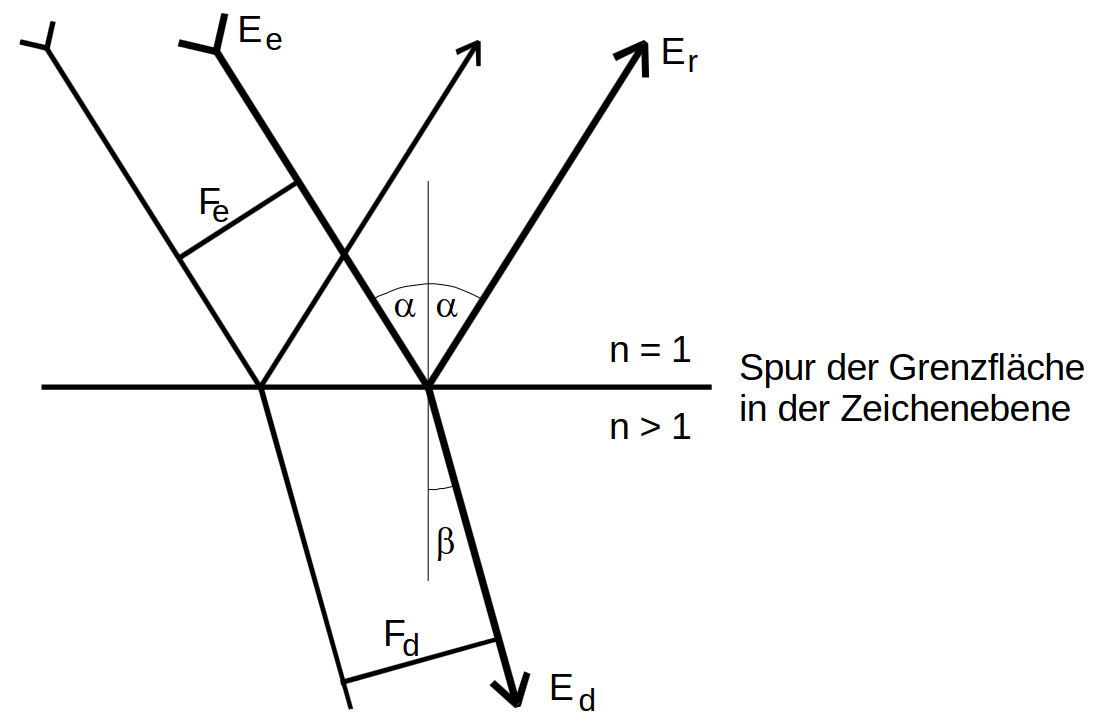
\includegraphics[height=5cm]{Grenzflaeche.png}
    \caption{Strahlengänge einer ebenen Welle an einer Grenzfläche\cite{Versuchsanleitung_v407}.}
    \label{fig:SkizzeGrenzflaeche}
\end{figure}

\noindent Die Tatsache, dass der Brechungsindex $n$ im Medium größer als 1 ist, impliziert bereits, dass die Lichtgeschwindigkeit $v$ im Medium kleiner ist als die
Vakuumlichtgeschwindigkeit $c$, was über die Beziehung $n = \sfrac{c}{v}$ leicht eingesehen werden kann. Nach dem \emph{Snelliusschem Brechungsgesetz} bedeutet dies 
ausßerdem, dass der Brechungswinkel $\beta$ kleiner als der Einfalls- bzw. Ausfallswinkel $\alpha$. Dementsprechend ändert sich auch der in der Abbildung 
\ref{fig:SkizzeGrenzflaeche} Querschnitt von $F_\text{e}$ auf $F_\text{d}$, was über trigonometrische Beziehungen den Energiesatz

\begin{equation*}
    S_\text{e}\cos(\alpha) = S_\text{r}\cos(\alpha) + S_\text{d}\cos(\beta) 
\end{equation*}

\noindent zur Folge hat. Über den im vorherigen Kapitel hergeleiteten Ausdruck für den Betrag des Poynting-Vektors \eqref{eqn:BetragS} ergibt sich 

\begin{equation*}
    c\varepsilon_0\vec{E}²_\text{e}\cos(\alpha) = c\varepsilon_0\vec{E}²_\text{r}\cos(\alpha) + v\varepsilon_0\vec{E}²_\text{d}\cos(\beta)
\end{equation*}

\noindent und unter Ausnutzung der Beziehung $n = \sfrac{c}{v}$

\begin{equation}
    \left(\vec{E}²_\text{e} - \vec{E}²_\text{r}\right)n\cos(\alpha) = \varepsilon\vec{E}²_\text{d}\cos(\beta).
\end{equation}


\section{Vorbereitung}

\section{Fehlerrechnung}
\end{document}